\chapter{Teoría del Aprendizaje}\label{sec:aa}
En este capítulo introduciremos los conceptos básicos del \ac{AA} para introducir posteriormente el concepto de \textit{Deep Learning}. Hablaremos del concepto de aprendizaje y de los diferentes tipos de problemas a los que se enfrenta el \ac{AA}

\section{Concepto de Aprendizaje Automático}
Un algoritmo de \ac{AA} es un algoritmo capaz de aprender información a partir de  un cierto conjunto de datos. Para saber de qué hablamos cuando hablamos de aprender podemos referirnos a \cite{mitchell-1997}, ``Un programa de ordenador se dice que aprende de una experiencia $E$ con respecto a un conjunto de tareas $T$ y medida de rendimiento $P$, si su rendimiento como tarea en $T$, medido con $P$, mejora tras conocer la experiencia $E$``. Desde el punto de vista de las tareas $T$, el \ac{AA} es interesante pues nos permite resolver una gran cantidad de tareas que son muy difíciles o incluso imposibles de resolver con programas escritos y diseñados por humanos, ya sea por el complejidad o por el tamaño de la tarea.

Otra definición interesante del concepto de aprendizaje es el de \cite{learningfromdata}. Para ello primero mencionamos los componentes del problema. Hay una entrada $x$, una función objetivo $f: \mathcal{X} \to \mathcal{Y}$, donde $\mathcal{X}$ es el espacio de todas las posibles entradas y $\mathcal{Y}$ es el espacio de los posibles resultados. Además, contamos con un conjunto de muestras $\mathcal{D} \subset \mathcal{X} \times \mathcal{Y}$ donde $y = f(x)$ si $(x, y) \in \mathcal{D}$. Finalmente, existe un algoritmo que usa el conjunto $\mathcal{D}$ para escoger una fórmula $g: \mathcal{X} \to \mathcal{Y}$ que aproxime $f$. Este algoritmo escogerá $g$ dentro de un conjunto de funciones $\mathcal{H}$.

\begin{figure}[!h]
    \centering
    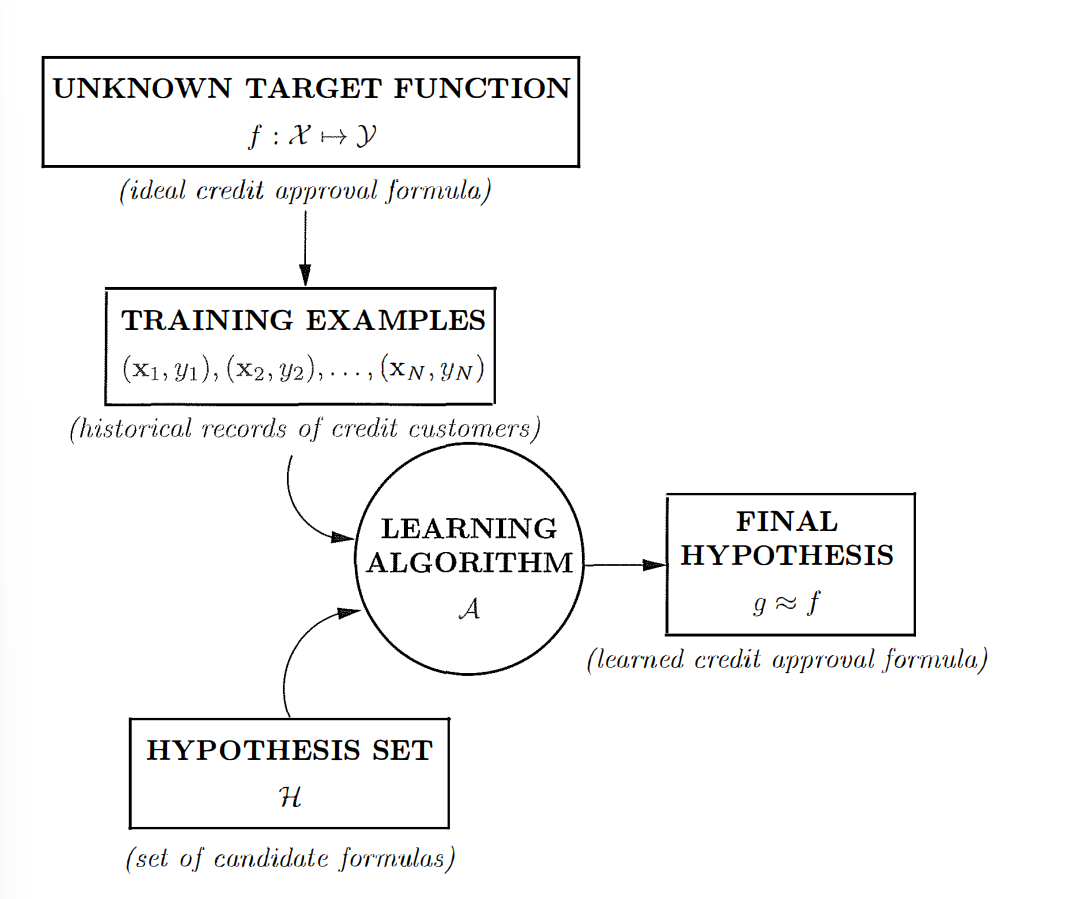
\includegraphics[width=0.8\textwidth]{figuras/learning.png}
    \caption{Escenario básico de un problema de aprendizaje. Fuente: \cite{learningfromdata}.}
    \label{fig:learningsetup}
\end{figure}

Si consideramos los múltiples componentes del problema, la función objetivo $f$ y las muestras de entrenamiento $\mathcal{D}$ están dictadas por el problema. Sin embargo, el algoritmo de aprendizaje y el conjunto de funciones en el que buscamos $\mathcal{H}$ no lo están, y son por lo tanto somos nosotros quienes las fijamos. Al conjunto $\mathcal{H}$ y al algoritmo se le refiere informalmente como el modelo de aprendizaje.

El \ac{AA} ha sido aplicado a una gran variedad de situaciones. En la literatura se pueden encontrar ejemplos:
\begin{itemize}
    \item Clasificación.
    \item Clasificación con valores perdidos.
    \item Regresión.
    \item Transcripción.
    \item Detección de anomalías.
    \item Predicción de valores perdidos.
    \item Estimación de densidad.
\end{itemize}

Con respecto a la medida de rendimiento $P$, esta debe de ser cuantitativa. La medida por excelencia en casos de clasificación es la precisión o \textit{accuracy}, definida como la proporción de muestras para las que el modelo ha producido una salida correcta. También en muchas ocasiones es útil la tasa de error, que mide la proporción de muestras para las que el modelo ha producido una salida incorrecta.

\section{Tipos de Aprendizaje Automático}
En función de la experiencia $E$, podemos clasificar los algoritmos de \ac{AA} en dos grandes grupos: algoritmos supervisados y no supervisados.
\begin{itemize}
    \item \textbf{Aprendizaje Automático No Supervisado}: cuando los datos con los que trabajamos están formados por un conjunto de datos que representa diferentes características de cada una de las muestras. Normalmente, en este caso el objetivo suele ser encontrar alguna propiedad importante para la estructura del conjunto. Un ejemplo clásico es el \textit{clustering} que consiste en agrupar los datos en subconjuntos que contengan características similares.
    \item \textbf{Aprendizaje Automático Supervisado}: cuando se tiene información de un conjunto con características y donde cada muestra tiene asociada una etiqueta. Así, el objetivo de estos problemas será encontrar la relación entre las características de una muestra y su etiqueta para poder etiquetar características futuras. Un ejemplo es el problema de clasificación.
    \item \textbf{Aprendizaje por Refuerzo}: cuando el conjunto de datos no contiene de manera explícita la salida correcta para cada entrada, sino que contiene una posible salida junto a una medida de como de adecuada esta salida es. Este tipo de aprendizaje es ideal para situaciones en las que no existe necesariamente un resultado correcto, como puede ser el problema de la conducción autónoma de vehículos.
\end{itemize}

\section{Problema de clasificación}

El problema de clasificación es el ejemplo más frecuente de aprendizaje supervisado. Consiste en, a partir de una población de entrada, clasificarla en diferentes subpoblaciones o clases. Se debe de conocer previamente el número de clases posibles, por lo que el problema consiste en decidir para cada elemento qué clase es la que mejor se ajusta a sus características observadas. Según el número de clases consideradas se puede distinguir entre:
\begin{itemize}
    \item \textbf{Clasificación Binaria}: cuando la clasificación se reduce a tan solo dos etiquetas. Se puede ver como un problema de verdadero o falso, o pertenencia o no a un subgrupo de la población.
    \item \textbf{Clasificación Multiclase}: cuando el conjunto de etiquetas es mayor que dos. En este caso se debe elegir entre todas ellas cuál es la más adecuada.
\end{itemize}

Nosotros nos centraremos en los problemas de clasificación multiclase.

\chapter{Fundamentos del Deep Learning}\label{sec:deep}
En este capítulo nos centraremos propiamente en el \textit{Deep Learning}. Para ello estudiaremos las redes neuronales prealimentadas, cómo funcionan y estudiaremos el aprendizaje basado en gradiente. Posteriormente hablaremos de redes convolucionales y concretamente de la arquitectura \texttt{EfficientNet}.

\section{Redes Neuronales Prealimentadas}
Las redes neuronales prealimentadas o \ac{MLP} son el modelo por excelencia del \textit{deep learning}~\cite{Goodfellow-et-al-2016}. El objetivo de un \ac{MLP} es el de aproximar una función $f^*$. Por ejemplo, para un clasificador, $y = f^*(x)$ lleva una entrada $x$ a una categoría $y$. Un \ac{MLP} define una correspondencia $y = f(x; \theta)$ y aprende el parámetro $\theta$ que lleva a la mejor aproximación de la función.

Este tipo de modelos se llaman prealimentados porque la información fluye a través de la función siendo evaluados desde $x$, a través de las computaciones intermedias usadas para definir $f$, y finalmente hasta el resultado $y$. Las redes prealimentadas son de vital importancia en el \ac{AA}, ya que son el fundamento de muchas aplicaciones comerciales. Por ejemplo, las redes convolucionales usadas para reconocer objetos en fotografías son un tipo especializado de redes neuronales prealimentadas.

Las redes neuronales prealimentadas son llamadas redes porque son normalmente representadas como la composición de muchas funciones distintas. Se asocia el modelo con un grafo acíclico dirigido describiendo cómo las funciones se componen entre sí. Por ejemplo, podemos tener tres funciones $f^{(1)}$, $f^{(2)}$ y $f^{(3)}$ conectadas de forma secuencial, para obtener $f(x) = f^{(3)}(f^{(2)}(f^{(1)}(x)))$. Esta estructura secuencial es la estructura más común usada en redes neuronales. En este caso, $f^{(1)}$ es conocido como la primera capa de la red, $f^{(2)}$ la segunda capa y así. La longitud total se conoce como la profundidad del modelo. El nombre \textit{deep learning} nace de esta terminología. La última capa se denomina capa de salida. Durante el entrenamiento de la red, intentamos que $f(x)$ se asemeje lo máximo posible a $f^*(x)$.

Por último, estas redes se llaman neuronales porque están ligeramente inspiradas en la neurociencia. La dimensión de cada capa oculta determina la anchura del modelo. Podemos ver cada capa como un conjunto de unidades que actúan en paralelo, cada una representando una función vector a escalar. Cada unidad recuerda a una neurona ya que recibe una entrada de otras unidades y devuelve su valor de activación.

Otra manera de entender las redes prealimentadas es comenzar con los modelos lineales y pensar en cómo solventar sus limitaciones. Los modelos lineales, tales como la regresión logística o lineal, son atractivos porque ajustarse eficientemente, ya sea de manera cerrada o mediante optimización convexa. Los modelos lineales también tienen el obvio problema de estar limitados a funciones lineales. Por lo tanto el modelo no puede entender la interacción entre dos variables cualesquiera de entrada.

Para extender los modelos lineales con el objetivo de representar funciones no lineales de $x$, en lugar de aplicar el modelo lineal a $x$ podemos aplicárselo a una transformación de la entrada $\phi(x)$, donde $\phi$ es una transformación no lineal. Nos podemos plantear en que transformación $\phi$ aplicar a $x$.

\begin{enumerate}
    \item Una opción es usar una $\phi$ muy genérica de dimensión muy alta, de manera que siempre tengamos capacidad suficiente para ajustar el conjunto de entrenamiento, pero la generalización al conjunto de evaluación suele ser bastante pobre.
    
    \item Otra opción es crear una $\phi$ de manera manual. Antiguamente este solía ser el método más común. Requiere una gran cantidad de trabajo humano para cada tarea y no son reutilizables.

    \item La estrategia que sigue el \textit{deep learning} es en aprender $\phi$. De esta manera, tenemos un modelo $y=f(x; \theta, w)=\phi(x;\theta)^Tw$. Ahora tenemos un conjunto de parámetros $\theta$ que usamos para aprender $\phi$ dentro de una clase amplia de funciones, y parámetros $w$ que llevan $\phi(x)$ a la salida deseada. Este es un ejemplo de red neuronal prealimentada, con $\phi$ definiendo una capa oculta. Esta técnica es la única de las tres que decide dejar de lado la convexidad del problema. 
\end{enumerate}

Este principio de mejorar modelos mediante el aprendizaje de características va mucho más allá de las redes neuronales prealimentadas y es un tema recurrente que se aplica a todo tipo de modelos en el \textit{deep learning}.

\section{Aprendizaje Basado en Gradiente}
La principal diferencia entre los modelos lineales que hemos visto hasta el momento y las redes neuronales es que la no linealidad de estas últimas hace que la mayoría de funciones de pérdida interesantes se vuelven no convexas. Es por esto que las redes neuronales normalmente se entrenan usando optimizadores iterativos basados en gradientes que simplemente llevan la función de coste o pérdida a un valor muy bajo. En la optimización convexa tenemos convergencia desde cualquier conjunto de parámetros iniciales, pero esto es algo que perdemos al usar métodos iterativos basados en gradiente.

\subsection{Funciones de Coste}
Es por esto, que un aspecto importante del diseño de una red neuronal profunda es la elección de la función de coste o pérdida. En la mayoría de casos, nuestro modelo paramétrico define una distribución $p(y | x; \theta)$ y por lo tanto aplicamos el principio de máxima verosimilitud. Esto significa usar la entropía cruzada entre los datos de entrenamiento y las predicciones del modelo como función de pérdida. 

En otras ocasiones, en lugar de predecir una distribución de probabilidad completa sobre $y$, simplemente predecimos algún tipo de estadístico de $y$ condicionado a $x$.

El función de coste total usada para entrenar una red neuronal normalmente combina una función principal con un término de regularización.

\subsection{Unidades de Salida}
La elección de la función de coste está íntimamente relacionada con la elección de la unidad de salida. La mayoría de ocasiones, simplemente calculamos la entropía cruzada entre la distribución de los datos y la del modelo. La elección de como representar la salida determina la forma de la función de entropía cruzada.

Cualquier tipo de unidad de red neuronal que puede ser usada como salida también puede ser usada como unidad oculta. Aquí, nos centraremos en el uso de estas unidades como salida del modelo, pero pueden ser usadas de forma interna también en un principio.

\paragraph{Unidades Lineales}\mbox{}\\
Un tipo sencillo de unidad de salida está basado en una transformación afín sin no linealidad. Normalmente se llaman unidades lineales.

Dadas características $h$, una capa lineal produce un vector $\hat{y}=W^Th + b$. Las capas de salida lineales normalmente se usan para producir la media de una distribución Gaussiana condicionada:
\begin{equation}
    p(y | x) = \mathcal{N}(y; \hat{y}, I)
\end{equation}

Maximizar el logaritmo de la verosimilitud es entonces equivalente a minimizar el error cuadrático medio.

\paragraph{Unidades Sigmoidales}\mbox{}\\
Muchas tareas requieren predecir el valor de una variable binaria $y$. Es decir, un problema de clasificación de dos clases. Podemos intentar definir una distribución de Bernoulli sobre $y$ condicionada a $x$. Como una distribución de Bernouilli está definida por tan solo un número, la red neuronal necesita predecir $P(y=1 | x)$. Para que este número sea una probabilidad válida, debe de estar en el intervalo $[0, 1]$.

Para esto usamos una función que siempre tiene un gradiente fuerte cuando el modelo se equivoca. Esta función es la función sigmoide definida como
\begin{equation}
    \hat{y} = \sigma(w^Th + b) = \frac{1}{1 + e^{-(w^Th + b)}}
\end{equation}

Podemos pensar en que la unidad de salida sigmoide tiene dos componentes. Primero, usa capa lineal y luego usa la función de activación sigmoide $\sigma$ para convertir la salida anterior en una probabilidad.

Vamos a omitir la dependencia sobre $x$ por un momento para discutir como definir una distribución de probabilidad sobre $y$ usando la salida de la capa lineal $z$. La función sigmoide puede ser motivada mediante la construcción de una distribución de probabilidad $\tilde{P}(y)$ no normalizada, es decir, que no suma 1. Por lo tanto podemos dividir por una constante apropiada para obtener una distribución de probabilidad válida. Si comenzamos asumiendo que el logaritmo de las probabilidad no normalizadas son lineales en $y$ y $z$, podemos usar la exponencial con el fin de obtener las probabilidad no normalizadas. Entonces normalizamos para ver que obtenemos una distribución de Bernoulli controlada por una transformación sigmoilad de $z$:
\begin{gather}
    \log \tilde{P}(y) = yz, \\
    \tilde{P}(y) = \exp{(yz)}, \\
    P(y)=\frac{\exp{(yz)}}{\sum_{y'=1}^1 \exp{(y'z)}}, \\
    P(y) = \sigma((2y - 1)z)
\end{gather}

La variable $z$ que define estas distribuciones sobre variables binarias se llama \textit{logit}.

\begin{figure}[h]
    \centering
    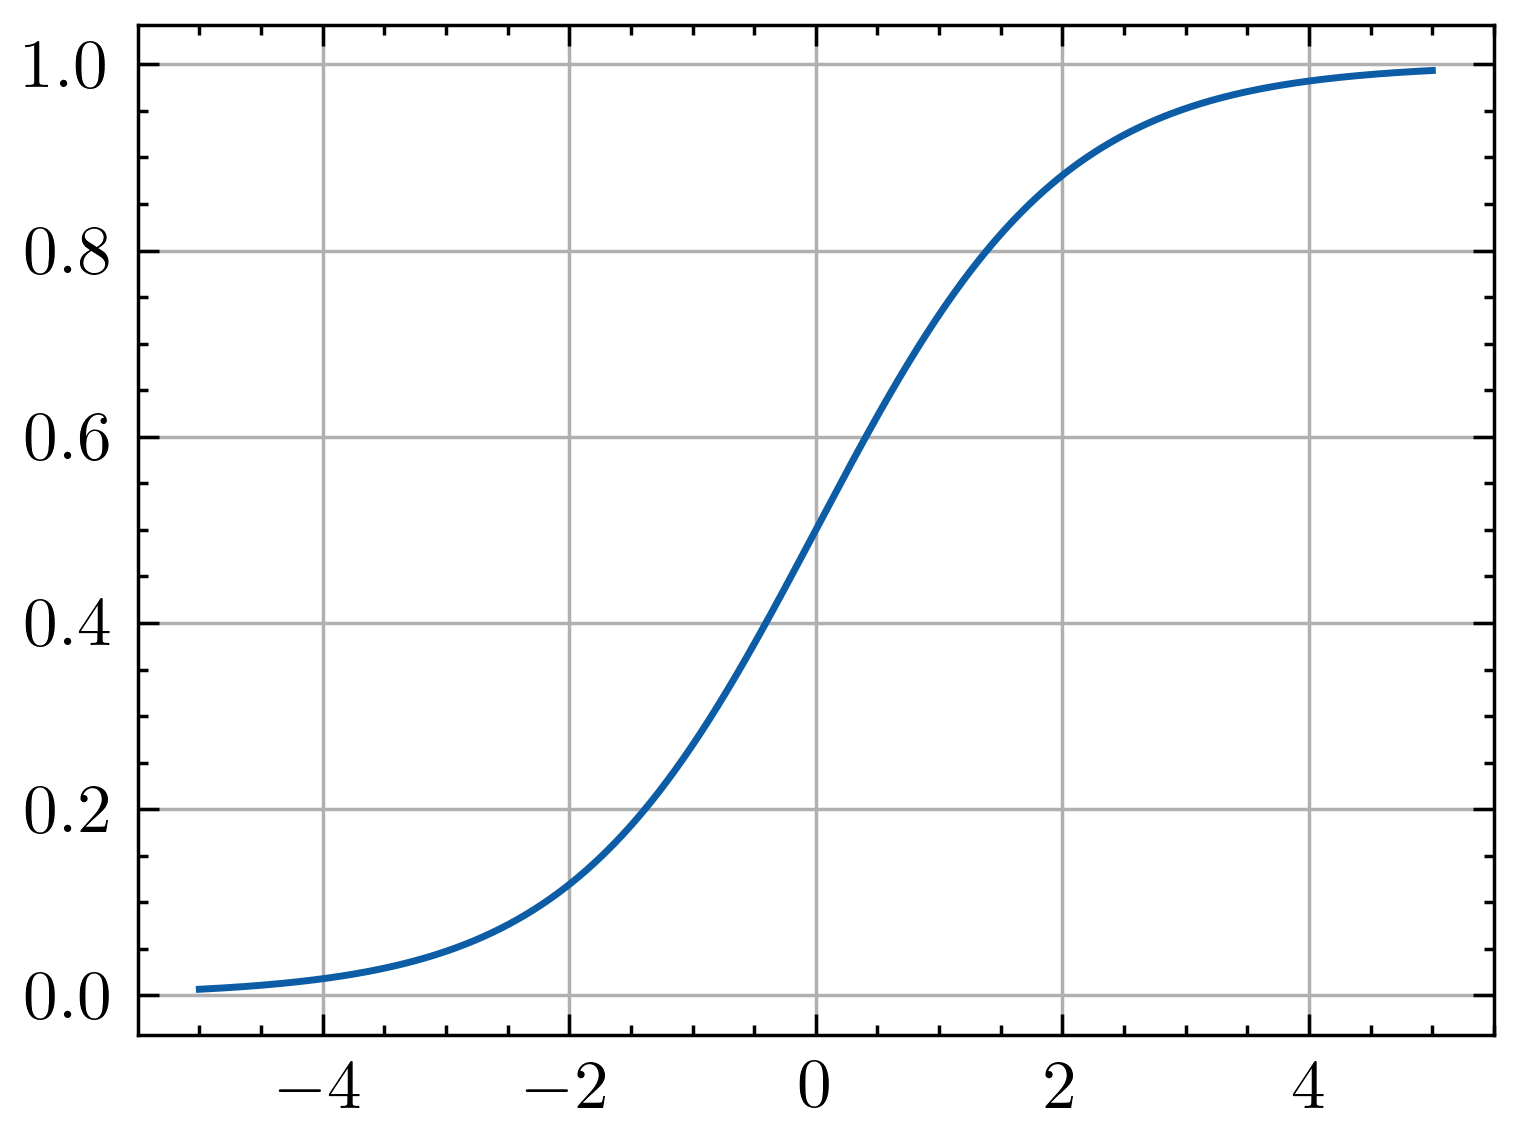
\includegraphics[width=0.8\textwidth]{figuras/sigmoid.png}
    \caption{Gráfica de la función sigmoide. Elaboración propia.}
    \label{fig:sigmoid}
\end{figure}


\paragraph{Unidades Softmax}\mbox{}\\

Cualquier momento que queramos representar una distribución de probabilidad sobre una variable discreta con $n$ valores posibles, usaremos la función \textit{softmax}. Puede ser vista como una generalización de la función sigmoide, que fue usada para representar una distribución de probabilidad sobre una variable binaria.

Para generalizar al caso de una variable discreta con $n$ valores, necesitamos producir un vector $\hat{y}$, con $\hat{y}_i=P(y=i|x)$. No solo necesitamos que cada elementos del vector esté entre 0 y 1, sino que además la suma de todo el vector sea igual a 1. Repitiendo el procedimiento usado para las sigmoides podemos generalizar la distribución. Primero, una capa lineal predice probabilidades logarítmicas no normalizadas:
\begin{equation}
    z = W^Th+b
\end{equation}
donde $z_i = \log \tilde{P}(y=i|x)$. Entonces, la función softmax puede exponenciar y normalizar $z$ para obtener $\hat{y}$. Formalmente, la función softmax está dada por: 
\begin{equation}
    softmax(z)_i=\frac{\exp{(z_i)}}{\sum_j \exp{(z_j)}}
\end{equation}

Al igual que en el caso de la función logística, el uso de la exponencial funciona bien cuando entrenamos el softmax para predecir el valor $y$ usando máxima verosimilitud.

\subsection{Unidades ocultas}
Como hemos mencionado anteriormente, cualquier unidad de salida que hemos explicado también puede ser aplicada como unidad oculta. Aún así, existen otras funciones de activación para este caso. Cabe destacar que la investigación sobre el diseño de las unidades ocultas sigue activo. Nosotros nos centraremos en algunas de las más comunes.

\paragraph{Unidades Lineales Rectificadas (ReLU) y sus generalizaciones}\mbox{}\\
Las unidades lineales rectificadas usan la función de activación $g(z)=\max \{0, z\}$. Son fáciles de optimizar porque son muy parecidas a las unidades lineales. La única diferencia es que estas devuelven cero en la mitad de su dominio. Esto permite que las derivadas mediante una unidad linear rectificada se mantengan grandes siempre que la unidad está activa. Los gradientes además son consistentes. Además, la segunda derivada de una ReLU es 0 casi en todo punto, y la derivada primera es 1 donde la unidad está activa.

\begin{figure}[h]
    \centering
    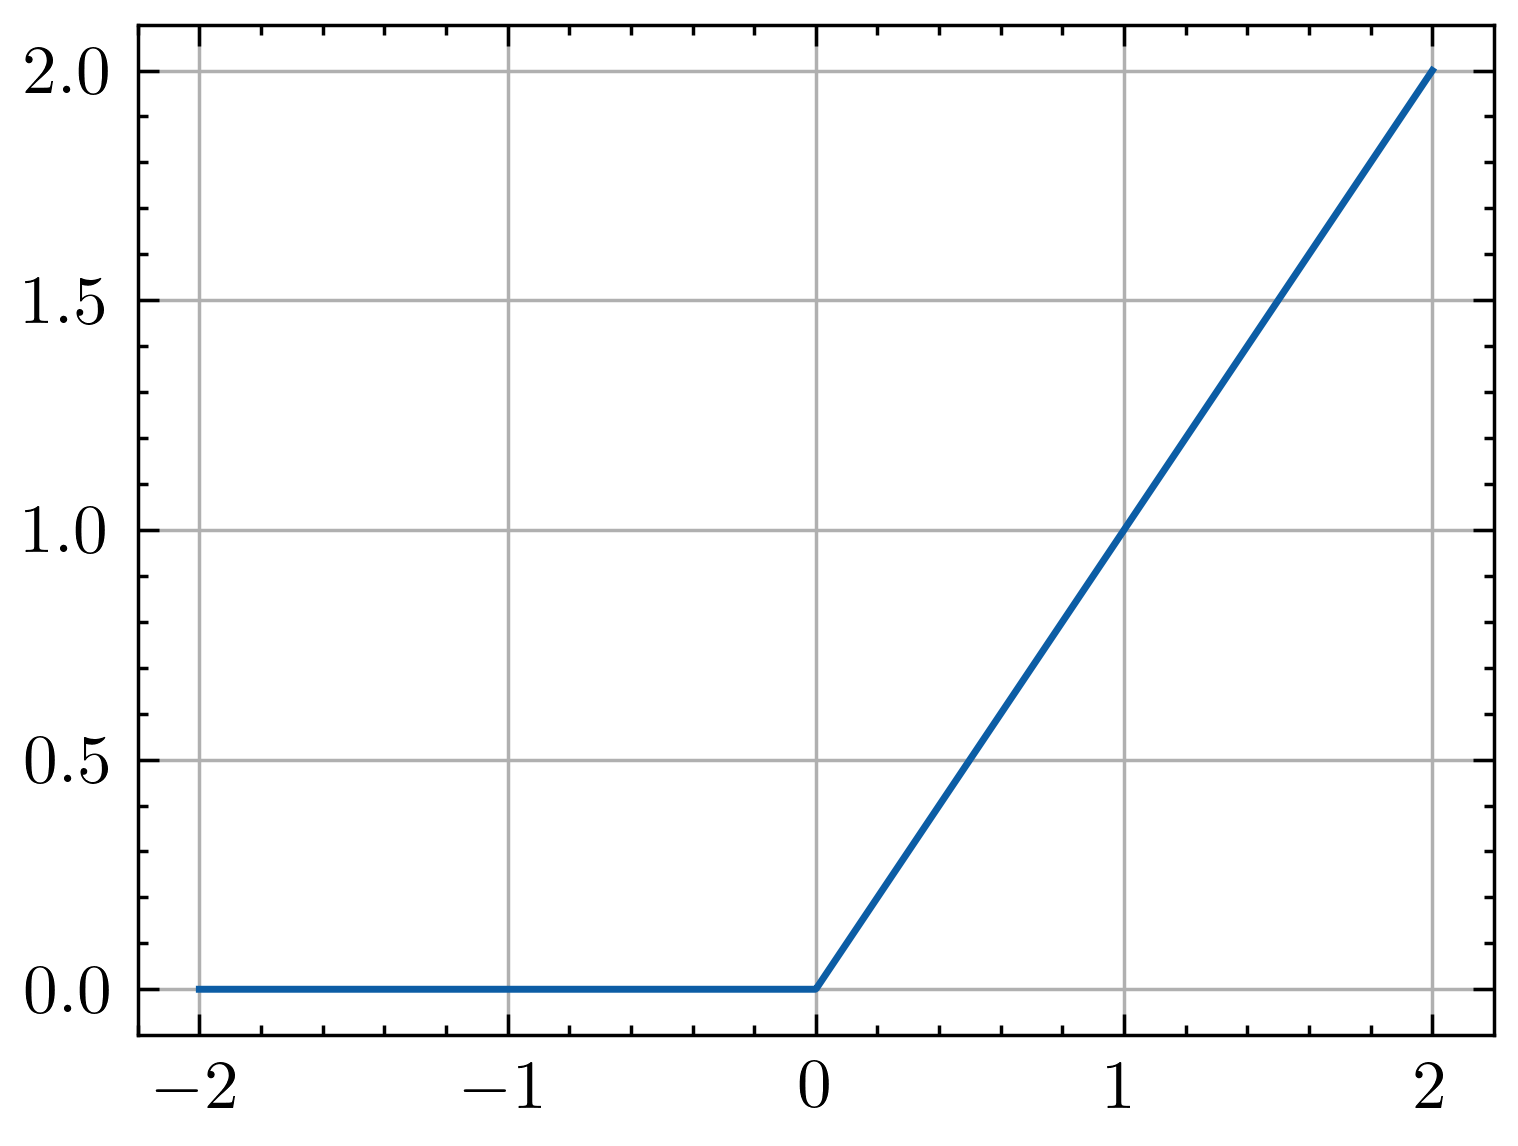
\includegraphics[width=0.8\textwidth]{figuras/relu.png}
    \caption{Gráfica de la función ReLU. Elaboración propia}
    \label{fig:relu}
\end{figure}

Existen bastantes generalizaciones de las ReLU. La mayoría de estas generalizaciones funcionan de manera comparable o incluso mejor que las primeras. Muchas generalizaciones se centran en solventar el problema de que no pueden aprender por descenso por el gradiente cuando su activación es cero.
\begin{itemize}
    \item \textbf{Rectificación de valor absoluto} consiste en fijar una pendiente de -1 cuando la salida de la ReLU es menor que 0, haciendo así $g(z)=|z|$.
    \item \textbf{Leaky ReLU} fija una pendiente muy pequeña como 0.01 cuando la salida de la ReLU es 0.
    \item \textbf{ReLU paramétrica} trata la pendiente ya mencionada como un valor a aprender.
\end{itemize}

\paragraph{Sigmoide Logística y Tangente Hiperbólica}\mbox{}\\
Antes de que se introdujesen las ReLU, la mayoría de redes neuronales usaban la función logística sigmoide como función de activación o la tangente hiperbólica.
\begin{gather}
    g(z) = \frac{1}{1 + e^{-z}} \\
    g(z) = \tanh{(z)}
\end{gather}

Estas funciones están estrechamente relacionadas pues $\tanh{(z)=2\sigma(2z)-1}$.

Ya hemos visto las unidades sigmoide como unidades de salida, usadas para predecir la probabilidad de que una variable binaria tome el valor 1. Sin embargo, las unidades sigmoidales se saturan en la mayor parte de su dominio, y solo son sensibles cuando su entrada es muy cercana a 0. La amplia saturación de las unidades sigmoidales hace que el aprendizaje por el gradiente sea muy difícil y es por ello que no se recomienda su uso como unidades ocultas. Solo se recomiendan cuando tengamos una función de coste capaz de deshacer la saturación de esta.

Las funciones de activación sigmoide son más comunes en otros escenarios que en \ac{MLP}. Las redes recurrentes, muchos modelos probabilísticos, y algunos \textit{autoencoders} tienen requisitos adicionales que hacen el uso de funciones sigmoidales más atractivos pese a la desventaja de la saturación.

\section{Redes Convolucionales}
Una \ac{CNN}~\cite{Goodfellow-et-al-2016} es un tipo especializado de red neuronal para procesar datos que tenga una topología de rejilla. Esto incluye datos en series temporales, que pueden ser pensados como una rejilla 1 dimensional a intervalos de tiempo regulares, e imágenes, que pueden ser pensadas como una rejilla 2 dimensional de píxeles. Las \ac{CNN} han demostrado ser realmente exitosas en múltiples aplicaciones prácticas. El nombre de ``red neuronal convolucional`` indica que la red hace uso de la operación de convolución. 

Vamos a explicar que es la convolución, cuál es la motivación para usarla en una red neuronal, descubriremos la técnica de \textit{pooling} que es usada a día de hoy en la mayoría de las redes convolucionales y nombraremos algunas redes importantes de este tipo.

\subsection{La Operación de Convolución}
En su forma más general, la convolución es una operación que toma como argumento dos funciones de variable real. Sean $f, g: \mathbb{R} \to {R}$ dos funciones de variable real, la convolución de ambas funciones se denota por $(f \star g)$ a su convolución y viene definida por:
\begin{equation}
    s(t) = (f \star g) = \int_{-\infty}^{\infty}f(s)g(t-s)ds
\end{equation}

Si usamos la terminología de las \ac{CNN}, nuestro primer argumento, es decir $f$ se le conoce como la entrada, y al segundo, $g$, será el núcleo o \textit{kernel} de la convolución. Al resultado en ocasiones se le llama mapa de características o \textit{feature map}.

Normalmente, cuando trabajamos con datos en un ordenador, no podemos tratar con un continuo sino con datos discretizados. Por lo tanto asumir que podemos evaluar las funciones en todo punto no es realista. Es por ello que definimos la operación de convolución discreta como será natural viendo la definición anterior:
\begin{equation}
    s(t) = (f \star g) = \sum_{s=-\infty}^{\infty}f(s)g(t-s)
\end{equation}

En el \ac{AA}, las entradas normalmente suelen ser tensores de datos, y el \textit{kernel} suele ser también un \textit{kernel} de parámetros que son adaptados por el algoritmo de aprendizaje que usemos. Debido a que cada elemento de la entrada y del \textit{kernel} debe de ser almacenado por separado, asumimos que estas funciones son cero en todos los puntos salvo en el conjunto finito del que almacenamos valores. En práctica, esto significa que podemos implementar la suma infinita como una suma finita de elementos de los tensores.

Además, también usaremos convoluciones sobre más de un eje a la vez. Por ejemplo, si usamos una imagen de dos dimensiones $I$ como entrada, posiblemente también consideremos usar un \textit{kernel} de dos dimensiones $K$:
\begin{equation}
    S(i,j) = (I \star K)(i,j) = \sum_m \sum_n I(m,n)K(i-m, j-n)
\end{equation}
Además, la convolución también es conmutativa por lo que podemos escribir también:
\begin{equation}
    S(i,j) = (K \star I)(i,j) = \sum_m \sum_n K(m,n)I(i-m, j-n)
\end{equation}
Normalmente se implementa la última fórmula pues hay menos variación en el rango de valores válidos de $m$ y $n$.

\subsection{Motivación}
La convolución implica tres ideas importantes que pueden ayudar a mejorar un sistema de \ac{AA}: compartir parámetros, interacciones dispersas y representaciones equivariantes. Además, también nos permite un método para trabajar con entradas de tamaño variable.

Las capas tradicionales de redes neuronales usan la multiplicación por una matriz de parámetros con un parámetro parámetro separado que describe la interacción entre cada unidad de entrada y cada unidad de salida. Esto significa que cada unidad de salida interacciona con cada unidad de entrada. Sin embargo, una \ac{CNN} suele tener interacciones dispersas. Esto es cuando el \textit{kernel} es más pequeño que la entrada (que suele ser el caso habitual). Por ejemplo, cuando procesamos una imagen, la imagen puede tener miles o millones de píxeles, pero podemos detectar características pequeñas pero útiles tales como bordes con \textit{kernels} que son del tamaño de cien píxeles o menos. Esto significa que necesitamos almacenar menos parámetros, lo que reduce requisitos de memoria y mejora la eficiencia estadística del modelo. También implica que calcular el resultado del modelo necesita de menos operaciones. Estas mejoras en eficiencia suelen ser bastantes grandes. Si hay $m$ entradas y $n$ salidas, entonces la multiplicación de matrices necesita de $m \times n$ parámetros y los algoritmos tendrán una complejidad de $O(m \times n)$. Si limitamos el número de conexiones con cada salida a $k$, entonces solo necesitaremos $k \times n$ parámetros. Para muchas aplicaciones prácticas, es posible obtener un buen rendimiento en la tarea de \ac{AA} mientras mantenemos $k$ órdenes de magnitud por debajo de $m$.

Compartir parámetros se refiere al uso de un mismo parámetro para más de una función en un modelo. En las arquitecturas tradicionales de redes neuronales, cada elemento de la matriz de pesos se usa exactamente una vez cuando se calcula la salida de una capa. En una \ac{CNN}, cada elemento del \textit{kernel} se usa en cada posición de la entrada (excepto quizás en el borde de esta). Que se compartan los parámetros significa que en lugar de aprender un parámetro para cada ubicación de la entrada se aprende únicamente un conjunto de ellos. Esto no afecta al tiempo de ejecución de un paso de la red, pero si disminuye los requisitos de memoria del modelo. Por lo tanto, las convoluciones son dramáticamente más eficaces que las matrices densas en términos de memoria y eficiencia estadística.

En el caso de la convolución, el hecho de compartir parámetros implica que la capa tiene una propiedad llamada equivarianza a translaciones. Decir que una función es equivariante significa que si la entrada cambia, la salida se mantiene igual. Formalmente, una función $f(x)$ es equivariante a una función $g$ si $f(g(x))=g(f(x))$. En el caso de la convolución, si $g$ es cualquier translación, esto es, desplaza la entrada, entonces la convolución es invariante a $g$. En el caso de imágenes, la convolución crea un mapa 2-D de dónde aparecen ciertas características en la entrada. Por ejemplo, es útil detectar bordes en la primera capa de una \ac{CNN}. Los bordes aparecen más o menos en todas las partes de la imagen, así que tiene sentido compartir los parámetros para toda la imagen. En algunos casos, si estamos procesando imágenes recortadas para estar centradas respecto a algo, como por ejemplo, la cara de una persona, tal vez no nos interese compartir parámetros.


\subsection{Pooling}

Una capa de una \textit{CNN} suele estar formada por tres etapas. En la primera etapa, la capa realiza convoluciones en paralelo para producir un conjunto de activaciones lineales. En la segunda etapa, cada activación lineal se ejecuta con una función de activación no lineal, tales como ReLU. En la tercera etapa, usamos una función de \textit{pooling} para modificar la salida de la capa.

Una función de \textit{pooling} reemplaza la salida de la red en una cierta localización con un estadístico de las salidas cercanas. Por ejemplo, el \textit{max pooling} consiste en calcular la salida máxima dentro de un entorno rectangular. Otras funciones de \textit{pooling} populares son calcular el promedio en un entorno rectangular, la norma $L^2$ de un entorno rectangular o la media ponderada basada en la distancia del píxel central.

En todos los casos, el \textit{pooling} nos ayuda a hacer una representación aproximadamente invariante a pequeñas translaciones de la entrada. La invariancia a translaciones locales puede ser una propiedad útil si nos interesa más la presencia de algunas características que el saber exactamente dónde están. Por ejemplo, para determinar si una imagen contiene un rostro, no necesitamos saber la posición de los ojos con una precisión perfecta, solo saber que hay un ojo izquierdo a la izquierda de la cara y un ojo derecho a la derecha de la cara.

Para muchas tareas, el \textit{pooling} es esencial para manejar entradas de tamaño variable. Por ejemplo, si queremos clasificar imágenes de un tamaño variable, la entrada a la capa de clasificación debe de tener un tamaño fijo. Esto normalmente se logra adaptando el tamaño de las regiones de \textit{pooling} de manera que la capa de clasificación siempre reciba el mismo número de características sin importar el tamaño de la entrada. Por ejemplo, la última capa de \textit{pooling} en una red puede estar definida para dar siempre cuatro características, una por cada cuadrante de la imagen, sin importar el tamaño de esta.

\section{EfficientNet}

Durante el desarrollo de este trabajo haremos uso de la arquitectura de \textit{EfficientNet}~\cite{efficientnet}. Esta arquitectura es un tipo de red convolucional centrada en escalar apropiadamente la profundidad, anchura y resolución de la red con el fin de obtener un mejor rendimiento.

\subsection{Escalado del modelo}
El problema que intenta resolver \textit{EfficientNet} es encontrar un buen factor de escalado entre la anchura, profundidad y resolución de la red. Para ello, primero se debe de formular el problema de forma teórica.

La capa $i$ de una red convolucional se puede definir como una función $Y_i=\mathcal{F}_i(X_i)$, donde $\mathcal{F}_i$ es el operador, $Y_i$ es el tensor de salida y $X_i$ es el tensor de entrada con forma $(H_i, W_i, C_i)$, donde $H_i$ y $W_i$ son las dimensiones espaciales y $C_i$ es la dimensión de los canales de la imagen. Una red convolucional se puede representar como una lista de capas compuestas: $\mathcal{N}=\mathcal{F}_k \circ \ldots \circ \mathcal{F}_2 \circ \mathcal{F}_1(X_1)$. En la práctica, muchas redes convoluciones se dividen en etapas y todas las capas en la misma etapa comparten la misma arquitectura. Por lo tanto se puede definir una red convolucional como:
\begin{equation}
    \mathcal{N}=\circ_{i=1,\ldots,s}F_i^{L^i}(X_{(H_i, W_i, C_i)})
\end{equation}

donde $F_i^{L_i}$ denota que la capa $F_i$ se repite $L_i$ veces en la etapa $i$. 

El objetivo de\textit{ EfficientNet}~\cite{efficientnet} consiste en expandir la longitud ($L_i$), anchura ($C_i$) y/o resolución ($H_i, W_i$) sin cambiar $\mathcal{F}_i$, la cual ya está previamente definida por una arquitectura base. Esto simplifica el problema de diseño pero sigue dejando un amplio espacio para explorar distintos parámetros para cada capa. Con el fin de reducir este espacio, los autores deciden restringir a que todas las capas deben de ser escaladas de manera uniforme con un ratio constante.

Los autores observan de manera empírica que las diferentes dimensiones en las que escalar no son independientes. Intuitivamente, para imágenes de mayor resolución, se debe de aumentar la profundidad de la red, con el fin de que campos receptores más grandes puedan ayudar a capturar características similares que incluyen más píxeles en imágenes más grandes. A su vez, también se debería de aumentar la anchura de la red cuando la resolución es mayor, con el objetivo de capturar patrones más finos con más píxeles. Por lo tanto se necesita coordinar y equilibrar las dimensiones sobre las que escalamos en lugar de escalar una única dimensión.

\subsection{La Arquitectura de EfficientNet}
Una vez dada la técnica de escalado para una red base, queda clara la importancia de esta última. Para obtener una arquitectura nueva, los autores han usado una búsqueda multi-objetivo de redes neuronales que optimiza tanto los \textit{FLOPS} como la precisión. Concretamente usando como función a optimizar $ACC(m)\times [FLOPS(m)/T]^\omega$ donde $ACC(m)$ es la precisión del modelo m, $FLOPS(m)$ los \textit{FLOPS} del modelo, $T$ el objetivo de \textit{FLOPS} a conseguir y $\omega=-0.007$ un hiperparámetro para compensar entre la precisión y los $FLOPS$. El resultado de esta búsqueda es un modelo llamado \texttt{EfficientNet-B0}. Aplicando posteriormente la técnica de escalado logran crear los modelos \texttt{EfficientNet-B1} hasta \texttt{EfficientNet-B7} siendo este último un modelo estado del arte en el momento de publicación de \cite{efficientnet}, siendo 8.4 veces más pequeña y 6.1 veces más rápida que la mejor red convolucional existente previamente.